\documentclass[pdftex,12pt,a4paper]{report}

% Some useful packages.
\usepackage{amsmath}
\usepackage{siunitx}
\usepackage{graphicx}
\usepackage{verbatim}
\usepackage{mhchem}
\usepackage{textcomp}
\usepackage{setspace}

% Reduces margins substantially.
\usepackage{geometry}
\newgeometry{margin=3.0cm}

% Allows headers and footers.
\usepackage{fancyhdr}
\pagestyle{fancy}
% Get rid of annoying line under header.
\renewcommand{\headrulewidth}{0pt}

% Properly fixed by installing texlive-fonts-recommended
% Temporary fix for missing font problem.
% N.B. I know this is wrong, but there is a problem with missing fonts otherwise.
% \renewcommand{\textdegree}{$^{\circ}$ }

\lhead{}
\chead{}
\rhead{}

\newcommand{\ts}{\textsuperscript}
\newcommand{\HRule}{\rule{\linewidth}{0.5mm}}

% Harvard style references.
\usepackage[backend=biber,style=authoryear,sorting=nyt,dashed=false]{biblatex}
\renewcommand*{\nameyeardelim}{\addcomma\space}
\addbibresource{references/references.bib} % note the .bib is required

% 12,000 words max.

% overall structure:
% Abstract
% Intro
% Data Sources
% Development of the Hurricane Detection Algorithm
% Conclusion
% Appendices
% References

% Common typos:
% possibly

\title{Objective Tracking and Classification of Hurricanes in the 20\ts{th} Century Reanalysis Dataset}
\author{Mark Muetzelfeldt - UCL Department of Geography}

\date{29 August, 2014}

\begin{document}

\begin{titlepage}

\begin{center}

\textsc{\LARGE University College London}\\[1.5cm]

\textsc{\Large MSc Environmental Modelling Dissertation}\\[0.5cm]

% Title
\HRule \\[0.4cm]
{ \LARGE \bfseries Objective Tracking and Classification of Hurricanes in the 20\ts{th} Century Reanalysis Dataset \\[0.4cm] }

\HRule \\[1.5cm]

% Author and supervisor
\begin{minipage}{0.4\textwidth}
\begin{flushleft} \large
\emph{Author:}\\
Mark \textsc{Muetzelfeldt}
\end{flushleft}
\end{minipage}
\begin{minipage}{0.4\textwidth}
\begin{flushright} \large
\emph{Supervisors:} \\
Dr.~Chris \textsc{Brierley} \\
Qinling \textsc{Wu}
\end{flushright}
\end{minipage}
\\[0.5cm]
29\ts{th} August, 2014
\\[0.5cm]

This research dissertation is submitted for the MSc Environmental Modelling at University College London


\vfill
% Bottom of the page

\end{center}

\end{titlepage}


\onehalfspacing
\section*{Abstract}

% Should be >= 400 words.
% Not included in word count.
% 255 words so far.
A procedure for the detection of hurricanes in the 20\ts{th} Century Reanalysis Project dataset is
developed. Tracks are derived from the dataset by tracking vorticity maxima over time. These derived
tracks are matched against best tracks taken from the International Best Track Archive for Climate
Stewardship (IBTrACS) best tracks dataset. Six different tracking configurations are evaluated:
using the vorticity at the \SI{995}{hPa} and \SI{850}{hPa} pressure levels and using the original
resolution data, data downscaled by cubic interpolation to two and three times the original
resolution. It is found that using downscaling to three times the resolution provides a better match
between the derived tracks and the best tracks. Tracks at the different pressure levels produce
similar results, and the \SI{850}{hPa} pressure level is chosen on theoretical grounds.

The derived tracks are used to obtain extra fields from the 20\ts{th} Century Reanalysis
Project dataset, such as the local minimum pressure and the temperature at the \SI{850}{hPa}
pressure level. These extra fields, along with the information obtained by matching the derived
tracks to the best tracks, are used to produce training and validation datasets for supervised
machine learning classification algorithms. Different classification algorithms are evaluated based
on classification success and error metrics. It is found that a Stochastic Gradient Descent
classifier combined with a simple threshold classifier produces the highest combined score on these
metrics.

The developed procedure is run over the course of the 20\ts{th} Century, and a comparison between
the estimated number of hurricanes and the number as recorded in the IBTrACS dataset is performed.
It is found that\dots

\begin{center}
\textbf{Word count:} TODO
\end{center}

\section*{Acknowledgements}

I would like to thank Dr. Chris Brierley for his guidance and assistance in this dissertation.
Technical expertise from Qinling Wu proved useful in setting the direction for this project.
Talking to Joshua Studholme helped to provide context for the field and ideas for analysis, as well
as giving me some pointers on extra-tropical transitions. % CLUMSY
Dr. Kevin Hodges (Reading University) provided many useful suggestions for the tracking algorithm.
Finally, numerous discussions with Robert Muetzelfeldt were invaluable for keeping me on track and
for sounding out various ideas.

\newpage

\tableofcontents

% Everything from here to auto-critique is included in word count.
\chapter{Introduction}
% From the dissertation handbook:
% Introduction, presenting the research problem, rationale, context and outline objectives,
% aims/objectives (possibly as a formal hypothesis).

% Rationale.
% ----------

% Impacts of hurricanes.
Hurricanes are one of nature's most impressive and devastating extreme weather events. The costliest
hurricane this century, hurricane Katrina, was responsible for 1833 deaths and caused \$108
billion USD in damage \parencite{TODOCITE}. % TODO: Need another sentence here.
Hurricanes are therefore of great importance socially,
economically and, in hurricane Katrina's case, even politically.

% Heat transport by hurricanes.
Hurricanes, and more generally tropical cyclones, are also known to be a major contributor to the
poleward heat flux that evens out the temperatures between the poles and the tropics, carrying an
estimated \SI{1.4e15}{W} towards the poles \parencite{emanuelContribution2012}. This
contribution is large enough that it may affect the thermohaline circulation
\parencite{huEffect2009}, a major component of the coupled atmosphere-ocean system of the Earth. So,
coupled with their socio-economic impact, understanding hurricanes is of intrinsic scientific
interest too, helping to understand the Earth's climate and to produce more accurate General
Circulation Models.

% Effects of global warming on frequency/intensity.
From a theoretical perspective, increasing global mean temperatures are predicted to lead to an
increase in the intensity of hurricanes \parencite{emanuelDependence1987}. This is backed up by
computer modelling, which predicts a 6\% increase in maximum wind speed under conditions of a rise
in global temperatures over the next 80 years \parencite{knutsonImpact2004}. Given that a
hurricane's destructive potential varies as the maximum surface wind speed cubed
\parencite{emanuelIncreasing2005}, this would lead to a 20\% increase in hurricanes' destructive
potential. In line with the theory, this destructive potential is found to have risen ``markedly''
since the 1970s \parencite{emanuelIncreasing2005}. As well as increases in the intensity of
hurricanes, increases in their frequency have been detected \parencite{goldbergRecent2001,
websterChanges2005, hollandHeightened2007}.

% Trends in hurricanes over time leading on to...
Most studies into hurricane frequency and intensity tend to rely on best tracks databases as their
primary data source, such as the IBTrACS database used in this study
\parencite{knappInternational2010}, or the tropical cyclone database from the National Hurricane
Center \parencite{jarvinianTropical1984}. These databases suffer from some problems when going into
the middle and early 20\ts{th} century, such as the lack of satellite data before the 1970s, and the
lack of reliable aeroplane reconnaissance data before the mid 1940s \parencite{changeNumber2007}.
Accordingly, in this study, the approach taken is a different one. Instead of using the numbers
compiled by various agencies as the primary source of information into hurricanes, the primary data
will be taken from reanalysis data, specifically the 20\ts{th} Century Reanalysis (20CR) Project
\parencite{compoTwentieth2011}.  Hurricanes will be detected in these data, and the detection
procedure will be trained and validated on recent data (from 1990 to 2009), where reliable best
tracks exist. Once the detection procedure has been trained, it can be used to run over the whole of
the 20\ts{th} century, providing an objective measure of the number of hurricanes in each year.

\section{Research Problem}
% Detection of hurricanes in 20CR dataset.
% * Reason: spans 20th C.
% * List other reanalyses that do not.
% * Problems with this dataset: low resolution, despite trying to make it objective, it will likely
% change over time, making trend detection tricky (laying groundwork for talking about this in
% discussion).

% Mention NCEP/NCAR Reanalysis 1
% Mention ERA-40
% Mention JRA-55

% BRIEF description of what reanalysis is,
A global reanalysis project is an attempt to reconstruct the complete historical state of the
atmosphere at a given spatial and temporal resolution, assimilating an incomplete series of
measurements of atmospheric variables (a more complete description is given in Section
\ref{sec:20crp}). Several reanalysis projects exist, such as NCEP/NCAR Reanalysis 1
\parencite{TODOCITE}, ECMWF ERA-40 \parencite{uppalaEra2006} and the JRA-55 \parencite{TODOCITE}.
These reanalysis only run for 66, 40 and 55 years respectively, and so would not be useful for
looking into hurricanes at the start of the 20\ts{th} century. The 20CR on the other hand covers
over 140 years, from 1871 to 2012, and is therefore suitable for studying the number of hurricanes
across the entire 20\ts{th} century.  It contains an estimate of the state of the atmosphere on a
T62 (2\textdegree) spatial resolution and at 6-hourly timesteps, with variables such as the
longitudinal and latitudinal wind speeds at the \SI{995}{hPa} pressure level and the temperature at
the \SI{850}{hPa} pressure level recorded.

\section{Existing Tracking and Detection Algorithms}
% Context.
% --------

% Tracking/detection: Literature review. Lots and lots of references.
% Tracking: why it's a good idea to track then detect. Links to Hodges 1 and 2.
% Detection: GCM:
% Talk about role of resolution
% Talk about
% Discuss different approaches.
% Detection: Reanalyses.
% List some previous attempts to detect hurr/tropical cyclones in reanalyses.
% Talk about the primary difference: the existence of best tracks datasets.

% TODO: Needs a bit of re-writing due to not being on the output of a GCM for reanalyses.
Several reasons exist for wanting to detect hurricanes in the output of GCMs. Often the goal is to
look into the effects of climate change with a warming climate \parencite{bengtsson1996, sugi2002,
yoshimura2006}. When running this sort of analysis, there is no objective measure of whether or not
an individual detection of a hurricane is correct or not, although often tests are done to make sure
that the resulting climatologies are realistic. This is in contrast to running the detection using
the output of a GCM that is part of a historical reanalysis dataset, where it is possible to match
the detected hurricane to a given tracks in a given best track database, as was done by
\textcite{walsh1995}.

% TODO: Ditto, make it clear that it's acting on global atm. output, not nec. GCM output.
There are two closely related approaches to detecting hurricanes in the output of GCMs. The first is
to examine the output of the GCM at every timestep, looking for a cell or cells which meet certain
criteria, and then produce tracks based on combining cells that meet these in criteria in different
timesteps. These criteria are normally involve vorticity at the \SI{850}{hPa} pressure level,
maximum wind speed, and temperature anomalies at different pressure levels. Additionally, the tracks
produced have to be longer than a certain time duration, typically 1.5 to 2 days. Examples of
studies that take this approach are \textcite{TODOCITEmultiple}. 

The second approach of detecting hurricanes is to first track some feature from one timestep to the
next (typically vorticity maxima), and then apply a set of criteria to each point in these tracks to
see whether they represent hurricanes or not. Normally, a time duration of the tracks must be longer
than a certain duration as well, again typically 1.5 days. These tracks can yield extra information
about the hurricanes, such as where their were formed, which is important in deriving details about
cyclogenesis \parencite{TODOCITE}. Useful information about the fate of the cyclone can also be
found, such as whether it undergoes an extra tropical transition \parencite{TODOCITE}. This is the
approach taken by \textcite{TODOCITE, hodges, camargo}, and is also the approach that will be used
in this study.

Both these approaches rely on thresholds being set for the criteria in advance of running the
detection procedure, although there may be some sensitivity analysis done on these thresholds as in
\textcite{walsh1995}. These thresholds can be somewhat arbitrary and can vary with resolution
\parencite{walsh2007}. Two studies that have looked at T63 resolution (very close to the T62 used by
the 20CR dataset), have used values of \SI{6e-5}{s^{-1}} as a threshold value for hurricanes in the
\SI{850}{hPa} vorticity \parencite{bengtsson2006, bengtsson2007}.  Therefore any value used in this
study should be of a similar magnitude to this number.  The thresholds can also vary from basin to
basin \parencite{camargo}, and thus need to be chosen quite carefully. 

This study takes a different approach to choosing these thresholds. Instead of deciding what they
should be before running the analysis, the analysis is run, and the values of e.g. vorticity and
temperature at the \SI{850}{hPa} pressure level are recorded for each point along each track. Due to
the matching of the tracks derived from the 20CR data and the best tracks, it is then possible to
see which values of these fields correspond to hurricanes, and which do not. This allows for setting
of the thresholds \textit{after} the bulk of the processing has been done, thus greatly speeding up
the process of finding optimum values for these thresholds. It also permits the use of machine
learning classification algorithms, which it is hoped will improve the accuracy of the hurricane
detection, as measured by the number of true and false positives. This is a similar approach to
\textcite{walsh1995}, who analysed the numbers of false and missing tropical cyclones over September
1989 and October 1992, and results of this study will be compared against these. It bears repeating
that this approach is only possible because this study is running the hurricane detection over a
historical reanalysis dataset, otherwise this would not be possible.

% Objectives/Project Structure.
% -----------------------------
% Outline of objectives for this project.
% Finish with a run-down of the structure of the rest of the dissertation, including why it deviates
% from the traditional Intro/Methods/Results/Discussion/Conclusion structure.
The objectives of this study are to develop a tracking algorithm that is capable of producing tracks
derived from the 20CR dataset that can be successfully matched to the tracks in the IBTrACS best
tracks database. Following from this, these derived tracks will be used to collect extra information for
each of the points in the track, such as temperature at \SI{850}{hPa}. This information will then
used, along with the information about whether a particular point corresponds with a hurricane or
not, to train different classification algorithms to correctly predict whether each point is a
hurricane or not. The classification algorithm which performs best on success and error metrics will
be chosen, and this process will form the hurricane detection procedure. This will then be run
over the course of the 20\ts{th} century, and aggregate statistics about the number of hurricanes
over this duration will be presented, along with a comparison between the estimated number of
hurricanes from the 20CR dataset and the IBTrACS database.

The following chapter will present more detail on the two data sources used in this study: the
20CR dataset and the IBTrACS database. Chapter \ref{chap:development} will then detail the steps
taken to develop the detection procedure, presenting a logical progression of the development along
with results pertinent to the following sections of the development. Chapter
\ref{chap:results_analysis} will then look into the results of running the procedure over the course
of the 20\ts{th} century. Chapter \ref{chap:discussion} will then discuss these results in the wider
context of hurricane detection and trends over the 20\ts{th} century, and Chapter
\ref{chap:conclusion} will provide a summary and conclusion of the findings. This deviates slightly
from the traditional thesis structure due to the time spent working on the detection procedure, and
the desire to present this development in a logical manner where the subsequent sections depend on
the results of the previous sections.

\chapter{Data Sources}

\section{20\ts{th} Century Reanalysis Project}
\label{sec:20crp}

% Key points:
% * Global reanalysis 1871-2012
% * Uses only SST, surf press, sea ice
% * Relatively bias free because of above (compared to say ERA-40)
% * spatio-temporal resolution
% * includes uncertainty
% * 56 ensemble members
The 20\ts{th} Century Reanalysis Project (20CR) is a project whose aim is to produce a consistent
best estimate of the state of the atmosphere by including information from a variety of different
sources using data assimilation \parencite{compoTwentieth2011}. Sea Surface Temperature (SST) and
sea ice data from the Hadley Centre Sea Ice and SST dataset \parencite{rayner2003} are used to drive
a GCM - the NCEP Global Forecast System \parencite{TODOCITE}. This is combined with pressure
observations from the International Surface Pressure Databank \parencite{TODOCITE}, which is
assimilated with the forecasts provided by the GCM by means of an Ensemble Kalman Filter (EKF). It
provides estimates at a 2\textdegree spatial resolution, and on a 6-hour timestep, from 1871 to 2012
(more years will be added using the same process in due time). A level of consistency is ensured by
using the same process from the beginning of the reanalysis to the end, and by using only SST, sea
ice and pressure data. This avoids the problems seen in other reanalysis projects, such as ERA-40
\parencite{TODOCITE}, which incorporate as much data as possible. This biases more recent years, as
e.g. satellite data from the 1970s onwards provides far more observations than exist before this
period. Due to the use of an EKF, it is also possible for the 20CR to provide estimates for the
uncertainty of each of its estimates at each timestep, although this information is not used as part
of this study.

% necessity of analysing single EM (ref compo2011)
The GCM and EKF are run with 56 ensemble members, meaning that for every timestep there are 56
estimates for the state of the atmosphere. According to \textcite{compoTwentieth2011}, individual
tracking of storms is best done through tracking them in individual ensemble members, instead of
looking at the ensemble mean. This is because the ensemble mean, in the presence of only a few
observations, exhibits less synoptic variability. % TODO: unclear, explain better.
Therefore the individual ensemble members were used in this study. Consequently, the analysis
carried out in this study had to be repeated 56 times, and this provides that classification
algorithms used in Section \ref{sec:classification} far more samples than would otherwise have been
the case.

\subsection{Technical Details}
% How it works:

% Runs a GCM - NCEP GFS - to produce background fields
% Technical details on GCM
The GCM used was the NCEP Global Forecast System \parencite{TODOCITE}, with parameterisation as
specified by \textcite{saha2006}. The version used in the reanalysis was slightly modified to permit
time varying \ce{CO2} and volcanic aerosols. These, along with incoming radiation, where specified
as in \textcite{saha2010}. The model was run at a horizontal resolution of T62 and a vertical
resolution of 28 vertical hybrid sigma-pressure levels \parencite{juang2005}. This horizontal
resolution is between the T42 and T106 resolutions analysed in \textcite{bengtsson1995}, and
therefore should be capable of producing hurricane-type vortices, as the T42 model in that study
was found to be capable of producing vortices, although it was noted that these vortices were of
lower intensity and that their overall structure was less realistic than in the T106 GCM. 

% Technical details EKF
The EKF is similar to the Monte Carlo approximation proposed by \textcite{evensen1994}. It is
'deterministic', and is based on the 'Ensemble Square Root Filter' of \textcite{whitaker2002}.

% Assimilates the observations and the output from the GCM using an EKF to provide an estimate as to
% the state of the atmosphere at each timestep
The process by which estimates are produced involves three main steps: 

\begin{enumerate}
    \item Spin up of GCM
    \item Assimilate pressure data using the EKF (repeated)
    \item Use GCM to predict the state of the atmosphere at the next timestep (repeated)
\end{enumerate}

56 individual GCMs are initialised with climatalogical states taken from 14 months before the start
of the production period, i.e. the period over which estimates are produced. The GCMs are then run
for 14 months, to ``reduce the effect of the initial condition in the lower layers of the land
model.'' This makes use of the SST and sea ice data. At this point, the 56 different states of the
atmosphere from the GCMs are used as background states for the EKF, which assimilates the pressure
observations for the current timestep, to produce 56 estimates for the state of the atmosphere based
on the GCM output and the observations. These estimates are then used as the starting point for the
GCMs, which predict what the state of the atmosphere will be in 6 hours time, and this is used as
the background state for the EKF, which assimilates the pressure observations at the new timestep. 

% Feeds this estimate back into the GCM to run another forecast
% Consistency of each EM not an issue (ref compo2011)
This continual predict and assimilate process repeats for 5 years, and the whole process is repeated
over the full course of the reanalysis period. It should be noted that this 5 year period leads to a
discontinuity in the data: every 5 years on the 1\ts{st} of January starting from 1876, the
individual ensemble members will not be continuous. This is not important for this study, because
there are very few hurricanes in the Atlantic over the December-January divide. However, it would be
more important if one were looking at tropical cyclones over the Pacific, when this is an active
period.

\subsection{International Surface Pressure Databank}
The pressure data comes from the International Surface Pressure Databank version 2 (ISPDv2)
\parencite{TODOCITE}. This takes its data from over 40 international agencies, and combines them
into one usable databank. One particularly notable data source is the IBTrACS dataset used in this
study (see Section \ref{sec:ibtracs}). This is of interest because this study treats these two data
sources as being independent, although this is not the case. However, due to the data assimilation
process, and all the other factors that go into making the reanalysis data such as the GCM and every
other source of pressure data, it is thought that the effect of this data being assimilated should
not overly affect the conclusions of this study. Indeed, in Section \ref{sec:TODO}, where a
comparison is made between a derived track and a best track, the surprising aspect is the degree to
which the pressures do not correlate, which suggests that the IBTrACS best track pressure data is
not solely responsible for the pressure along the track's course.

% Results summary and usage for hurricane detection:
% * compo2011
% * neff2013
% * emanuel2010

\subsection{Representations of Hurricanes in the 20CR dataset}

In \textcite{neff2013}, the path of the Galveston Hurricane of the 8\ts{th} September, 1900 is
analysed. The analysis finds that the hurricane is detectable through a minimum in the pressure
field, even though the mean pressure field was used. They find that the track derived from the 20CR
for this hurricane was systematically to the north-east of the corresponding best track (taken from
the IBTrACS dataset). However, this study points to the fact that even hurricanes as far back as the
beginning of the 20\ts{th} century are well represented. Figure \ref{fig:TODOFIG} shows the pressure
and vorticity fields for one ensemble member and one date of this hurricane. In this figure, the
2\textdegree resolution of the data is clearly visible, as is the vorticity maximum and the pressure
minimum.

% Figure showing Galveston Hurricane.

In a more comprehensive study, \textcite{emanuel2010} used an earlier version of the 20CR dataset to
look at tropical cyclone activity from 1908-1958. He used dynamical downscaling (i.e. using a
high resolution model with the 20CR data providing boundary conditions for this model, not to be
confused with the simple cubic spline interpolation downscaling used in this study) to better
represent the structure of the tropical cyclones. He found a ``marginally significant increase'' in
the number of northern hemisphere tropical cyclones, along with a high correlation between the power
dissipation index from derived from the 20CR reanalysis and the best tracks from the same period.

% TODO: is this necessary? Maybe appendix?
% Format and availability:
% * NetCDF4
% * (individual results available as GRIB)
% * nersc portal

\section{IBTrACS Best Tracks Dataset}
\label{sec:ibtracs}
The International Best Track Archive for Climate Stewardship (IBTrACS)
\parencite{knappInternational2010} aims to be a homogenised global collection of best tracks of
tropical storms and tropical cyclones. It collects best tracks from numerous Regional Specialized
Meteorological Centers (RSMCs) and Tropical Cyclone Warning Centres (TCWCs), and combines these
together, removing duplicates and trying detect common discrepancies, such as dates being different
by one day and the positions between tracks not being the same. 

% TODOIMPROVE: chapter title?
\chapter{Development of the Hurricane Detection Procedure}
\label{chap:development}

% Overall description to go here, with flow chart.
% Mention:
% * project URLs
% * choice of tracking then classification vs classifying individual CDPs
% * amount of processing required

\begin{figure}[hbp]
    \centering
    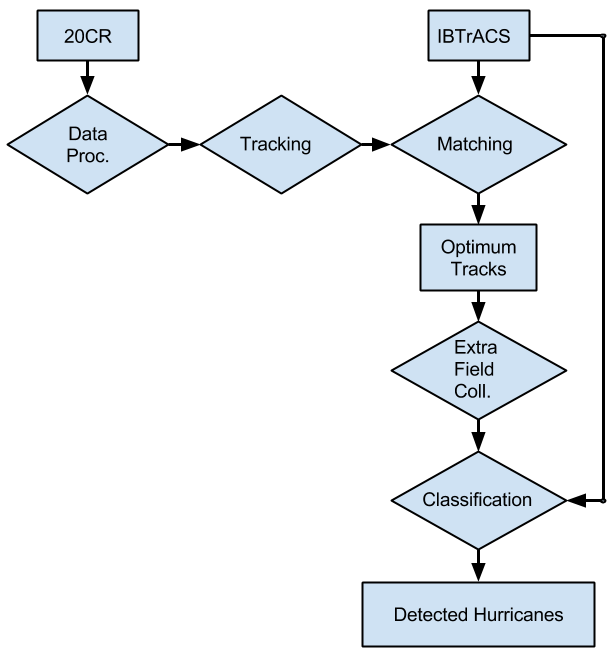
\includegraphics[width=\textwidth]{figures/hurricane_detection_procedure}
    \caption{Flowchart showing the steps in the hurricane detection procedure.}
    \label{fig:hurricane_detection_proc}
\end{figure}

\section{Data Processing}

\subsection{Wind Fields and Vorticity}

In the 20CR data, the longitudinal and latitudinal wind fields, $u$ and $v$ respectively, were used
to calculate the vorticity and wind speeds. These are available at three different pressure levels:
\SI{995}{hPa}, \SI{850}{hPa} and \SI{250}{hPa}. The \SI{250}{hPa} fields were only used to determine
whether or not they were suitable for tracking of hurricanes, and it was found that they did not
produce suitable tracks, and were not further used (see Section \ref{sec:results_tracking}). The
formula for vorticity, $\omega$, is given by:

\begin{equation}
    \omega = \frac{\partial v}{\partial x} - \frac{\partial u}{\partial y}
    \label{eqn:vorticity}
\end{equation}

The surface of the earth, $R_e$, is taken as its mean radius of \SI{6371}{km}, and $\phi$, $\lambda$
denote the latitude and longitude coordinates in radians. $u_{i, j}$ denotes the longitudinal wind
speed at grid cell $i, j$. Then $\omega$ can approximated on the surface of the Earth using a
2\ts{nd} order approximation: %CLUMSY

% Calculation in code is a little different because it uses degrees instead of radians:
% More like vorticity = du / (2 * dlon * cos(lat * pi / 180) * Earth_circ / 360) - dv / ((2 * dlat) * Earth_circ / 360)

\begin{equation}
    \omega \approx \frac{\Delta v}{2 \Delta x} - \frac{\Delta u}{2 \Delta y} = \frac{v_{i,j+1} - v_{i,j-1}}{2 R_e \cos{\phi} \Delta \lambda} - \frac{u_{i+1,j} - u_{i-1,j}}{2 R_e \Delta \phi }
    \label{eqn:vorticity_2nd_order}
\end{equation}

The vorticities at the \SI{995}{hPa} and \SI{850}{hPa} levels were calculated.

\subsection{Maxima and Minima detection}
\label{sec:methods_maxima_minima}

% TODO: Define PSL higher up?
For the vorticity fields, maxima are of primary interest as these represent grid cells where the
wind is rotating most strongly. Conversely, for the PSL field, minima are of primary interest. A
maximum or minimum was defined as a cell whose value was greater or less than all eight of its
surrounding cells. Vorticity maxima play a vital role in deriving tracks from the 20CR data, and
pressure minima are useful both for comparison with the best tracks data and classification of the
tracks.

\subsection{Downscaling of Data}

Following \textcite{TODOCITEhodgesXXX}, the vorticity field was downscaled to a finer resolution. This was
done so as when tracks were derived from these data, the so called ``staircase effect'', whereby
tracks are seen to follow the grid cells at the resolution of the 20CR data, was minimised (an
example of this ``staircase effect'' can be seen in Figure \ref{fig:katrina_individual_match_em7}). This
downscaling was accomplished using a cubic spline interpolation, and the data were downscaled to two and
three times their original resolutions. The efficacy of this downscaling will be demonstrated in
Section \ref{sec:results_tracking}.

\subsection{Data Processing Results}

Figure \ref{fig:katrina_data_proc} shows the progression of the data from its raw form, to a derived
vorticity, and then a downscaled to three times the original resolution vorticity field. Figure
\ref{fig:katrina_max_mins} shows an example vorticity and pressure field taken from around Hurricane
Katrina, and the corresponding maxima for the vorticity and minima for the pressure fields.
TODOWRITE:
say interesting things about these figures.

\begin{figure}[hbp]
    \centering
    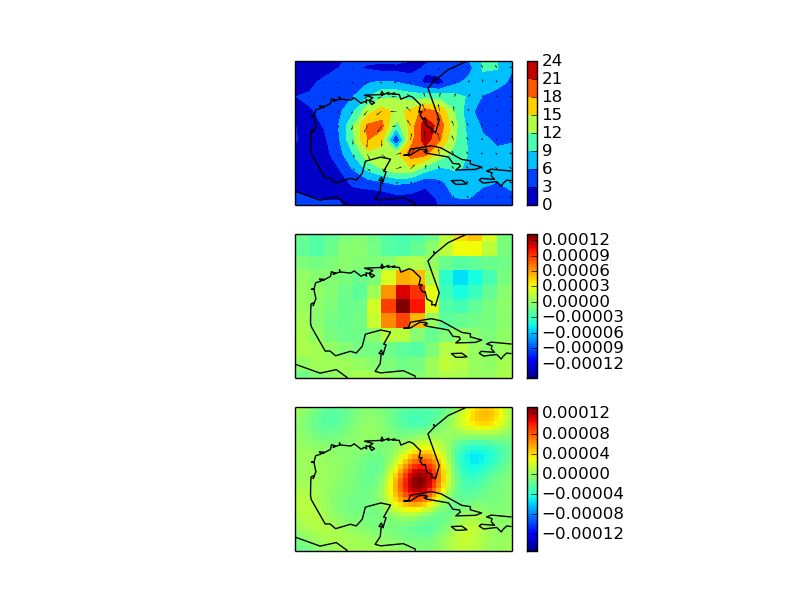
\includegraphics[width=\textwidth]{figures/katrina_data_proc}
    \caption{TODOWRITE: Caption goes here.}
    \label{fig:katrina_data_proc}
\end{figure}

\begin{figure}[hbp]
    \centering
    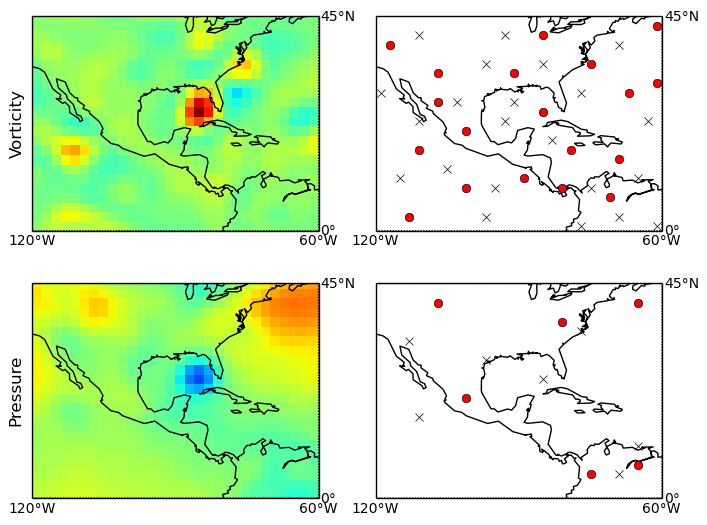
\includegraphics[width=\textwidth]{figures/katrina_max_mins}
    \caption{TODOWRITE: Caption goes here.}
    \label{fig:katrina_max_mins}
\end{figure}

\section{Tracking}

From both initial experimentation, and reading the literature \parencite{TODOCITEmultiple}, it was found
that tracking on minima of the pressure field did not produce suitable tracks for identifying
storm systems. This was due to the pressure field being subject to synoptic scale disturbances
that mean that minima may not be present due to the surrounding gradient of this field. Whilst it is
possible to apply high pass filtering to remove these disturbances, it was decided to follow
\textcite{TODOCITEmultiple} and produce derived tracks from the 20CR data based on vorticity maxima.

% TODOIMPROVE: This section is confusing on re-reading it. I think I need to make it clearer that I'm going to
% compare different configurations.
For each timestep, the vorticity maxima were calculated, as per Section
\ref{sec:methods_maxima_minima}. This was done for both the \SI{995}{hPa} and \SI{850}{hPa} pressure
levels, and for the one, two and three times the actual 20CR resolution, yielding a total of six
possible configurations for the tracking. These various configurations were compared, and the
results can be seen in Section \ref{sec:results_tracking}. Maxima that were below a cutoff value
of \SI{2.5e-5}{s^{-1}} were not used as part of the tracking algorithm, as these represent weak maxima
that are unlikely to be part of even tropical storms. This choice is revisited in Section TODOREF where
some further justification is given for this value.

The tracking algorithm used was a simple nearest neighbour tracking algorithm, with a modification
that counted two or more vorticity maxima that were sufficiently close as being part of the same storm
system, with the location and strength of the maximum given by the strongest of
these maxima. This cutoff distance was set as eight times the distance between the cells at
0\textdegree N, or approximately \SI{1800}{km}. This distance was found to reduce problems of
vorticity maxima merging and splitting. The algorithm worked as follows:

%  TODOIMPROVE: flowchart?
\begin{enumerate}
    \item Detect all vorticity maxima for the first timestep. If two maxima are less than the cutoff
        distance apart, combine both maxima, taking the strength and position of the strongest of
        the two maxima
    \item Make each of the vorticity maxima in the first timestep the beginning of a derived track
        (whose length could end up being only one)
    \item Detect all vorticity maxima in the second timestep, combining close weaker maxima into
        stronger. % TODOIMPROVE: not totally clear that I'm talking about the combining step here.
    \item Calculate nearest neighbour in the second timestep to first timestep, and set this as the
        next member of the derived track
    \item Move onto the third timestep and repeat the process
\end{enumerate}

Whilst this algorithm is considerably less sophisticated that that of \textcite{hodges1994}, it was
found to produce sufficiently good tracks to pick up most of the best tracks in the IBTrACS dataset,
and almost all of the best tracks that were hurricanes (Section  \ref{sec:results_tracking}). A
discussion of other tracking algorithms can be found in Section \ref{sec:discussion_tracking_algs}.

\subsection{Tracking Results}
\label{sec:results_tracking}

Once tracks have been derived from the 20CR, it is possible to match them to the corresponding best
tracks. The corresponding best track must be close the derived track in space, and its temporal
duration must overlap the duration of the derived track. In this project, an overlap of 6 timesteps,
or one and a half days, was required for there to be a match between a derived track and a best
track. Additionally, the mean distance from the derived track and the best track had to be lower
than a given threshold, taken as \SI{500}{km}. An example of a matching derived track taken from
one ensemble member and best track is shown in Figure \ref{fig:katrina_individual_match_em7}.
% N.B. em7 is counting from 0.
This shows how the cumulative and mean distances between a derived track (from ensemble member 8)
and a best track are calculated. All matching tracks across all the ensemble members for each of the
different configurations for Hurricane Katrina are shown in Figure
\ref{fig:katrina_six_tracking_configs}. This shows a typical hurricane that makes landfall. Some
noticeable points from this figure are TODOWRITE.

\begin{figure}[hbp]
    \centering
    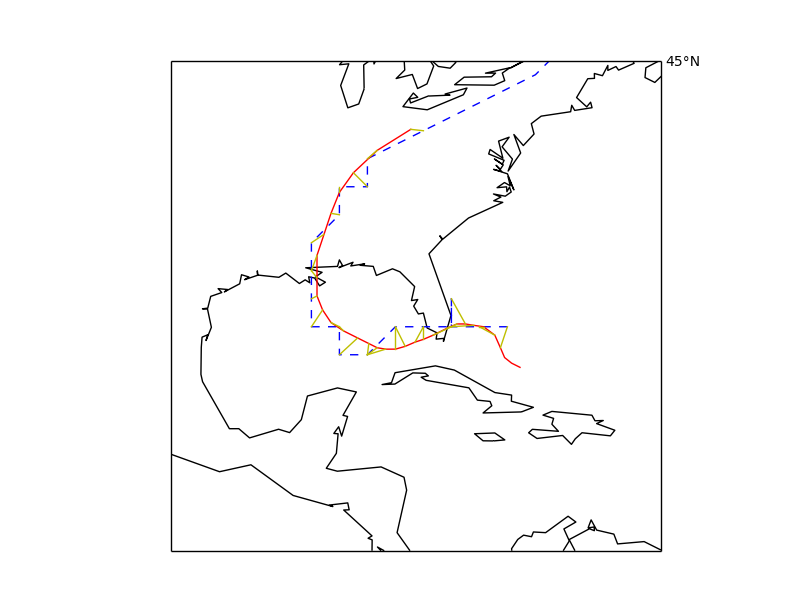
\includegraphics[width=\linewidth]{figures/katrina_individual_match_em7}
    \caption{Individual match between best track (red) and derived track (blue dashed) for Hurricane
        Katrina. The derived track was generated from the \SI{850}{hPa} pressure level using the
        original resolution and ensemble member 8. The match between the best track and the derived
        track is shown using yellow lines, which show the distance between the two tracks at each
        timestep. The cumulative distance is the sum of these distances, and the mean distance is
        the cumulative distance divided by the number of matches.
    }
    \label{fig:katrina_individual_match_em7}
\end{figure}

\begin{figure}[hbp]
    \centering
    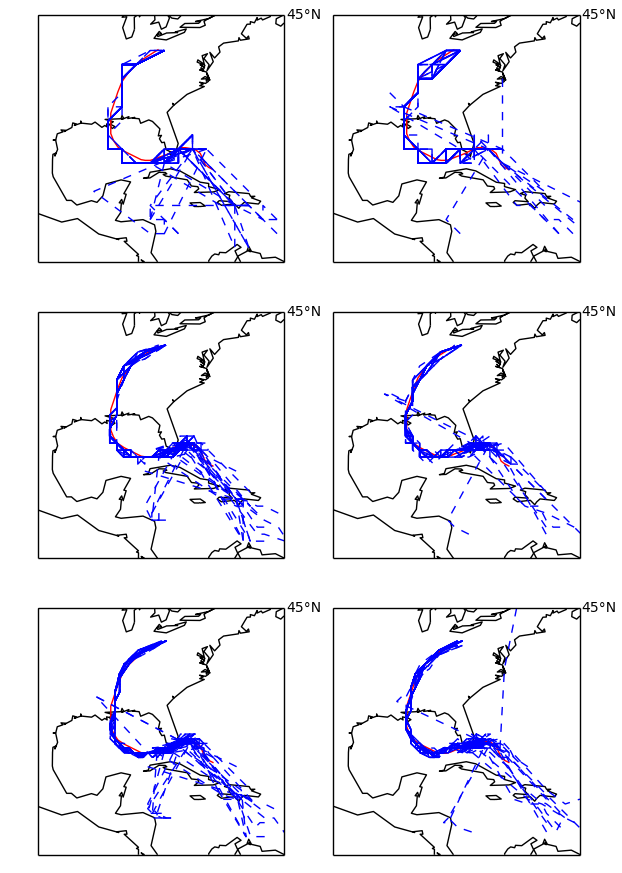
\includegraphics[width=\linewidth]{figures/katrina_six_tracking_configs}
    \caption{Caption goes here.}
    \label{fig:katrina_six_tracking_configs}
\end{figure}

To judge the tracking ability of the different tracking configurations, this matching across all
best tracks and derived tracks was done for each year in the ten year period 2000-2009.
% TODOIMPROVE: switch to cumoveroverlap as it is much easier to describe.
For each year, the combined average distance between each derived track and best track was
calculated. This number was divided by the total number of matches, so as a particular configuration
that achieved relatively few matches would be penalised. This produces a metric by which the various
configurations can be judged, and each of the configurations was then compared the others to see how
they performed on this metric. The results of this comparison can be seen in Figure TODOFIG. It is clear
that higher resolution, downscaled data produces better tracks that the unscaled data. This suggests
that for tracking, scaling of three times the original resolution should be used. What is less clear
is which is better: the \SI{995}{hPa} or the \SI{850}{hPa} pressure levels. TODOWRITE: why I picked
\SI{850}{hPa}.

% TODOFIG XX: Comparison of wins/losses of different tracking configurations.

\newpage
\section{Extra Field Collection}

Up until this point in the processing, only the $u$ and $v$ wind fields have been utilised. From
these, the vorticity has been calculated and tracks have been derived from the maxima of these
fields.  However, to successfully classify part of a track as being of hurricane strength, it is
necessary to collect more fields. These fields will help to distinguish hurricanes from
non-hurricanes. To this end, the latitude, longitude, date and ensemble member were used to obtain
further variables from the 20CR dataset. These variables were:

\begin{enumerate}
    \item \textbf{Minimum pressure:} the pressure minimum within \SI{1000}{km} of the vorticity
        maximum was found and the distance from the vorticity maximum to this minimum was also stored.
    \item \textbf{Ambient pressure difference:} the difference in pressure between the minimum
        pressure and the local mean pressure, as calculated by taking the surrounding 121 grid cells
        and averaging their pressures.
    \item \textbf{Temperature at \SI{995}{hPa}:} the temperature at the \SI{995}{hPa} pressure
        level.
    \item \textbf{Temperature at \SI{850}{hPa}:} the temperature at the \SI{850}{hPa} pressure
        level.
    \item \textbf{Temperature difference:} the temperature difference between the \SI{995}{hPa} and
        \SI{850}{hPa} pressure levels.
    \item \textbf{Maximum windspeed:} the maximum wind speed in the nearest 121 grid cells.
    \item \textbf{CAPE:} TODOWRITE
    \item \textbf{PWAT:} TODOWRITE
    \item \textbf{RH995:} TODOWRITE plus mention that is was found not to be that useful, and so dropped.
\end{enumerate}

Figure XX shows the pressure and vorticity fields surrounding the vorticity maxima for the Hurricane
Katrina track (taken from ensemble member YY). Figure XX shows the different fields plotted for each
timestep that Katrina was tracked for. Figure XX shows the derived pressure and maximum wind speed
for Katrina, plotted with the equivalent variables for the matching best track. From this figure, it
is clear that there is very little correlation in these two variable between the derived track and
% Check this\dots
the best track. This is surprising, not least because the 20CR assimilates the pressure data from
the IBTrACS dataset. Reasons as to why this might be so are examined further in XXX.

% TODOFIG XX: one timestep per day showing wind/vorticity for Katrina.

% TODOFIG XX: plot of all collected fields for Katrina.

% TODOFIG XX: plot showing poor correlation between Katrina derived and best.

\section{Classification}

% TODOWRITE: Need to mention supervised/unsupervised machine learning. In fact, need to mention machine
%learning full stop!
% TODOWRITE: mention fields I have collected are termed features in machine learning terminology.
% TODOWRITE: mention that CDPs are equivalent to samples in machine learning terminology.

% Description of the goal of classification and how it applies in this setting. Set out terminology
% that I am going to use.
% standard by which the various classifiers can be trained/judged.
Now that for each ensemble member a number of tracks have been derived from the 20CR data, and that
extra fields have been collected using the track's positions at different timesteps, it is possible
to use this information to classify each point of each track as either being a hurricane or not.
These points will be knows as cyclone data points (CDPs) and for a typical year there are around
100000 of these points, spread across the 56 ensemble members.

Classification is the process of taking a dataset and splitting it up into various categories based
on the attributes of each item in the dataset. For the purposes of hurricane classification, this is
a binary classification, i.e. a CDP is either a hurricane or it is not. More fine-grained approaches
are possible, such as splitting each CDP into a category from the Saffir-Simpson hurricane scale,
but in this analysis the only concern was trying to correctly categorise whether or not a given CDP
was a hurricane.

Given that each derived track has also been matched to a best track, it is also possible to use the
information from the best tracks dataset about whether the point on the best track is a hurricane or
not as an objective standard for whether or not the corresponding point on the derived track
represents a hurricane. This is represented visually in Figure TODOFIG, which shows every CDP for the
year TODOFIG, as well as whether the individual point has been matched to a hurricane in the best
tracks dataset or not. In classification terminology, this matching represents the gold standard by
which the classification algorithms can be trained, and by which their performance can be validated.
This allows classification algorithms to take the information derived from the 20CR and perform
classification based on this information.

% TODOFIG showing CDP with training set info included.

\subsubsection{Classification Successes and Errors}

% Explanation of FPs and FNs, TPs and TNs. Talk about Gold standard and how I am using IBTrACS as a
% gold standard. Relationship to Type I/II errors (maybe). Venn diagram showing FP/FN/TP/TN.

When classifying data with a binary classifier for which a gold standard exists, there are four
possible results of an individual classification. These are:

\begin{enumerate}
    \item \textbf{True Positive (TP):} The classification predicts that the CDP is a hurricane and
        this is verified by the best tracks information.
    \item \textbf{True Negative (TN):} The classification predicts that the CDP is not a hurricane
        and this is verified by the best tracks information.
    \item \textbf{False Positive (FP):} The classification predicts that the CDP is a hurricane and
        this is refuted by the best tracks information.
    \item \textbf{False Negative (FN):} The classification predicts that the CDP is not a hurricane
        and this is refuted by the best tracks information.
\end{enumerate}

When classifying a dataset, the collection of these results can be represented visually with a Venn
diagram, as shown in Figure TODOFIG. They can also be represented in tabular form in an Error Matrix
(also called a Contingency Table or Confusion Matrix). An example of an Error Matrix can be seen in
Table TODOTABLE, which shows the successes and failures of a simple classifier for a subset of the data.

\subsubsection{Sensitivity, Positive Predictive Value and False Positive Rate}

From the success and error results, various metrics are defined that give a measure of how well a
particular classifier performs at various tasks. Of these metrics, three will be considered in this
project:

\begin{enumerate}
    \item \textbf{Sensitivity:} This is defined as $\frac{TP}{TP + FN}$. In this context, it gives a
        measure of how many hurricanes are correctly detected from all the actual hurricanes. 1
        represents a perfect sensitivity.
    \item \textbf{Positive Predictive Value (PPV):} This is defined as $\frac{TP}{TP + FP}$. In this
        context, it gives a measure of how many of the predicted hurricanes from the classification
        algorithm are actually hurricanes. 1 represents a perfect PPV.
    \item \textbf{False Positive Rate (FPR):} This is defined as $\frac{FP}{FP + TN}$. In this
        context, it gives a measure of the detection rate of all actual hurricanes. 0 represents a
        perfect FPR.
\end{enumerate}

Sensitivity is often plotted against FPR to make a Receiver Operator Characteristic plot (ROC plot).
ROC plots are useful for determining which particular classifier performs best over a given training
and validation dataset. The top left corner of this plot represents perfect classification.  Another
plot which will be utilised in this project is a plot of Sensitivity against PPV, which will again
be used to determine which of the classifiers performs best. This plot is more useful in the context
of this project, as for the given datasets, very high values of FP detection are seen, which means
that the FPR will typically be very low, and less information can be gleaned from this particular
metric. Also, as will be explained in the next section, the Sensitivity and the PPV can be used to
obtain an estimate of the number of actual hurricanes. Examples of these plots can be seen in
Figures TODOFIG and TODOFIG.

\subsubsection{Estimate of the Number of Actual Hurricanes}

When any of the classifiers is run on a dataset, it will produce a prediction of which of the
members of that dataset are hurricanes, $H_{predicted}$. The PPV value derived for that particular classifier will
allow an estimate of the number of TPs for that prediction. Likewise, from the estimated number of
TPs, the sensitivity will allow a means of estimating the number of actual hurricanes, $H_{est. actual}$,
in the dataset. The equation for this is:

\begin{equation}
    H_{est. actual} = \frac{PPV \times H_{predicted}}{sensitivity}
    \label{eqn:n_actual_hurricane}
\end{equation}

\subsection{Classifiers}

\subsubsection{Threshold Classifier}
% How this is related to a Decision Tree classifier, how it was optimised.
The threshold classifier is the simplest of the classifiers considered. It works by using different
values for thresholds for one or more of the collected fields for each CDP. Any CDPs which have
field value which are e.g. higher than the specified threshold are considered hurricanes, and any
which are lower or equal to the threshold are considered not hurricanes. Despite its simplicity,
good results are possible with the threshold classifier by judicious choice of the thresholds for
each of the fields. These thresholds were first picked manually, then a simple brute force search
was carried out for values on either side of the chosen values. The metric for success was the sum
of the sensitivity and the PPV for the given classifier, where a larger value is better (a value of
2 would be perfect for this metric). It is also very easy to configure this classifier so as to
increase the sensitivity or PPV, although there is a trade-off between these two metrics, as shown
in Figure TODOFIG.

This classifier is a simple version of a decision tree classifier, which passes the incoming data
through a series of binary tests, determining which category a particular CDP should end up in based
in the results of these tests.

The approach of using thresholds is very similar to the approach taken by
\textcite{walshObjective1997}. The main difference between his approach and the one here is that in
this case the thresholds are applied after the processing has been done, thereby allowing far more
scope for experimenting with changes to these threshold values (i.e. the whole processing step does
not have to be run to experiment with different threshold values). This allows for a much faster
retrieval of optimum thresholds with regard to a given metric, although it comes at a cost of having
to run the data analysis in a way that gathers fields for all of the CDPs without being able to
discard fields based on whether or not they pass a particular threshold test.

% Plot of sens/PPV for varying vorticity threshold.

\subsubsection{Linear/Quadratic Discriminant Analysis Classifiers}

% How these work.
For binary classification, Linear Discriminant Analysis (LDA) and Quadratic Discriminant Analysis
(QDA) are two closely related classification algorithms that allow computationally cheap
classification of data where a gold standard is available under trained supervision.
\textcite{TODOCITE} gives a full account of both approaches, and a brief description of how they
work will be given here. The principal idea is to calculate the mean and covariance for all the
features of each group of data: $\mu_1$, $\sigma_1$ and $\mu_2$, $\sigma_2$. $\mu_1$ will lie at the
heart of the first group of features, and $\sigma_1$ will give a measure of the spread of this group
amongst each of the feature axes, and likewise for the second group. LDA then finds the dividing
surface between the two means (a plane in the same number of dimensions as there are features) based
on the relative values of the two variances. QDA is similar except that the dividing surface is
governed by a quadratic equation, and thus affords greater discriminating power between the two
groups.

These algorithms were not implemented from scratch; instead the implementations in the Python
library scikit-learn were used \parencite{scikitLearn2011}.

\subsubsection{Stochastic Gradient Descent Classifiers}
% TODO: Need to explain what samples are higher up.
% How this works.
Stochastic Gradient Descent (SGD) classifiers are an efficient class of classifiers that can scale
to 2 million samples, and are thus suitable for the problem in this project. This makes them more
suitable than e.g. a Support Vector Machine classifier, which only scales to around \SI{10e5}{}
samples.  They work by TODOWRITE.

Again, the scikit-learn implementation for this classifier was used \parencite{scikitLearn2011}.
% TODO: Explain feature scaling.
This particular classifier is sensitive to feature scaling, therefore the input features must be
scaled before the classifier is trained with this dataset, and likewise any data to be classified
must be scaled using this same scaling. Dataset scaling was provided by the scikit-learn library.

\subsubsection{Combining Classifiers}
With some of the classifiers, it was clear from examination of the output that they performed well
apart from producing FPs in areas of e.g. low vorticity or low temperature at \SI{850}{hPa}.
Therefore it made sense to combine the output of e.g. an SGD classifier with a threshold classifier.
The result of this is to reduce the number of FPs, and increase the number of TNs by the same
amount. This has the effect of increasing the PPV and FPR, but has no effect on the sensitivity.

\subsection{Classifier Performance}

% Explain how 20 years worth of data were split into a training/validation dataset.

% Figures showing performance of various classifiers in terms of FP/FN/TP/TN for 3 variables plotted
% against vorticity for training set. Discussion of performance differences.

\subsubsection{Training Dataset}
For the training dataset, all tracks from all ensemble members from the even years between 1990 and
2008 were taken. Given that each track is comprised of multiple (at least six) CDPs, this leads to a
large number of samples. On average, there were TODOCHECK samples per year, leading to a total
sample size of TODOCHECK million samples. This training dataset was used as a way of picking optimum
values for the threshold classifier manually (as defined by a maximum combined value of sensitivity
and PPV), and then using a brute force around the chosen values to verify that these values were
indeed the local maximum. The training dataset was also used to train each of the LDA, QDA and SGD
classifier.

\subsubsection{Validation Dataset} The validation dataset was similarly made up of all the tracks
from all ensemble members from the odd years between 1991 and 2009. This ensured that the training
and validation datasets were independent. It had a similar number of samples as the training
dataset: TODOCHECK million samples.

\chapter{20\ts{th} Century Analysis Results}
\label{chap:results_analysis}
% Data analysis and results.

\chapter{Discussion}
\label{chap:discussion}

\section{Tracking Algorithms}
\label{sec:discussion_tracking_algs}.

\chapter{Conclusions}
\label{chap:conclusion}

% Not included in word count.
\addcontentsline{toc}{chapter}{Auto-critique}
\chapter*{Auto-critique}

% Harvard style bibliography.
\addcontentsline{toc}{chapter}{References}
\printbibliography[title={References}]

%\appendix
%\section{Additional information}

\end{document}
